\section{Definizione}

Il sistema operativo è quel programma che è \textbf{sempre in esecuzione} quando il computer è acceso, questo viene anche detto il \textit{kernel}, il suo compito è di gestire le interazioni tra l'utente e l'hardware del computer su cui opera.

\spacer
Dato che il sistema operativo si interfaccia direttamente con l'hardware è importante comprendere a fondo la struttura dei moderni computer quali CPU, memoria e dispositivi di I/O. È infatti responsabilità del sistema operativo allocare queste risorse ai programmi.

\spacer
Assieme al \textit{kernel} ci sono altri due tipi di programmi:
\begin{sitemize}
    \item I \textbf{programmi di sistema}, che fanno parte del sistema operativo, ma non sono necessariamente parte del kernel.
    \item Le \textbf{applicazioni}, ovvero tutti i programmi che non sono associati al sistema operativo.
    \item Il \textbf{middleware}, esclusivo ai sistemi operativi per dispositivi mobile, permette di semplificare lo sviluppo delle applicazioni fornendo una collezione di ambienti software per gli sviluppatori.
\end{sitemize}

\begin{figure}[H]
    \centering
    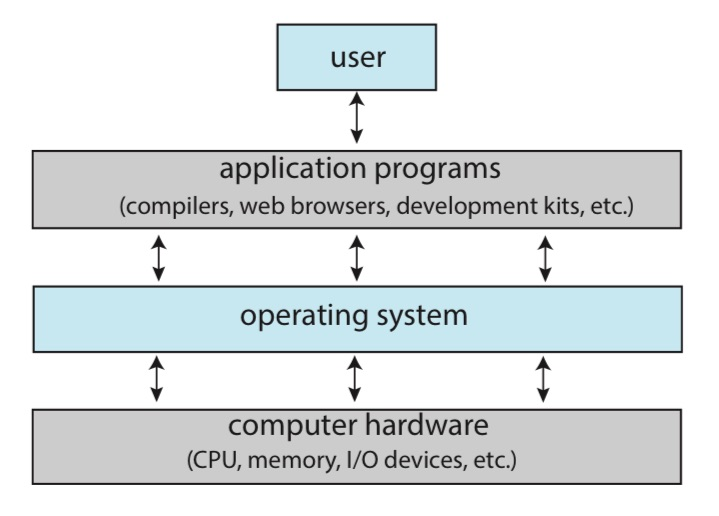
\includegraphics[width=0.45\linewidth]{assets/image.jpeg}
\end{figure}

Il sistema operativo ha diversi compiti rispetto all'utente e all'hardware, questo significa che deve bilanciare prestazioni e semplicità di utilizzo.

\subsubsection*{Lato Utente}
Il sistema operativo deve \textbf{massimizzare le prestazioni} che vengono attribuite a uno o più utenti in modo che esso possa completare il lavoro più velocemente.

\subsubsection*{Lato Hardware}
Dal punto di vista dell'hardware il sistema operativo ha il compito di \textbf{allocare le risorse} ai programmi dell'utente, \textbf{gestire eventuali errori} hardware e software e deve limitare l'utilizzo improprio delle risorse.

\subsection{Modello a Gusci Concentrici}
La struttura del sistema di calcolo può essere schematizzata mediante un "modello a cipolla" o a gusci concentrici.

I gusci circondano l'hardware, ogni livello propone al successivo un'interfaccia di sempre più alto livello, fino ad arrivare all'interfaccia utilizzata dagli utenti.

\begin{figure}[H]
    \centering
    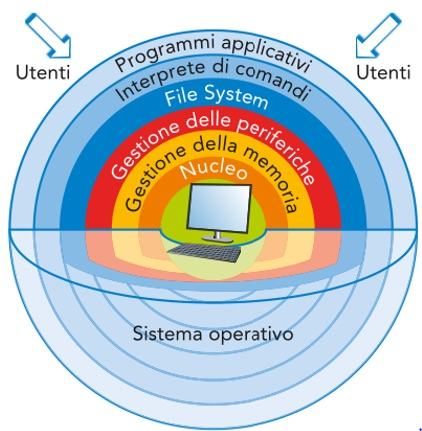
\includegraphics[width=0.35\linewidth]{assets/modello-gusci-concentrici.jpeg}
\end{figure}

\subsection{Avvio}
All'accensione il computer compie una serie di operazioni per arrivare al sistema operativo:

\begin{note}
    \textbf{Legacy BIOS}
    \begin{enumerate}
        \item \textbf{BIOS (\textit{Basic I/O System}):}
              Si trova nella ROM del computer ed è il primo ad essere avvisto.
              esegue check del componenti hardware.
              fornisce una serie di funzioni di base per l'accesso all'hardware
        \item \textbf{MBR(\textit{Master Boot Record}):}
              Il Bios cerca nei dischi un bootloader a cui passare il controllo.
              Questi, se presenti, si trovano nei primi 512 byte del disco, ovvero l'MBR.
        \item \textbf{Boot Loader:}
              Ha al compito di inizializzare il kernel e, di conseguenza, il sistema operativo. Alcuni esempi sono GRUB per linux e BootX per macOS.
    \end{enumerate}
\end{note}

\subsubsection*{UEFI BIOS}
\begin{enumerate}
    \item \textbf{BIOS UEFI (\textit{Unified Extensible firmware Interface})}
    \item \textbf{EFI Boot Loader:}
          Sostituisce MBR e Bootloader, si trova su una partizione del disco di avvio (identificata dalla flag boot)
          Carica Kernel a Sistema operativo
\end{enumerate}
